% Copyright © 2012 Martin Ueding <dev@martin-ueding.de>
%
% Copyright © 2012 Martin Ueding <dev@martin-ueding.de>
%
\documentclass[11pt, ngerman, fleqn]{scrartcl}

\usepackage{graphicx}

%%%%%%%%%%%%%%%%%%%%%%%%%%%%%%%%%%%%%%%%%%%%%%%%%%%%%%%%%%%%%%%%%%%%%%%%%%%%%%%
%                                Locale, date                                 %
%%%%%%%%%%%%%%%%%%%%%%%%%%%%%%%%%%%%%%%%%%%%%%%%%%%%%%%%%%%%%%%%%%%%%%%%%%%%%%%

\usepackage{babel}
\usepackage[iso]{isodate}

%%%%%%%%%%%%%%%%%%%%%%%%%%%%%%%%%%%%%%%%%%%%%%%%%%%%%%%%%%%%%%%%%%%%%%%%%%%%%%%
%                          Margins and other spacing                          %
%%%%%%%%%%%%%%%%%%%%%%%%%%%%%%%%%%%%%%%%%%%%%%%%%%%%%%%%%%%%%%%%%%%%%%%%%%%%%%%

\usepackage[activate]{pdfcprot}
\usepackage[left=3cm, right=2cm, top=2cm, bottom=2cm]{geometry}
\usepackage[parfill]{parskip}
\usepackage{setspace}

\setlength{\columnsep}{2cm}

%%%%%%%%%%%%%%%%%%%%%%%%%%%%%%%%%%%%%%%%%%%%%%%%%%%%%%%%%%%%%%%%%%%%%%%%%%%%%%%
%                                    Color                                    %
%%%%%%%%%%%%%%%%%%%%%%%%%%%%%%%%%%%%%%%%%%%%%%%%%%%%%%%%%%%%%%%%%%%%%%%%%%%%%%%

\usepackage{color}

\definecolor{darkblue}{rgb}{0,0,.5}
\definecolor{darkgreen}{rgb}{0,.5,0}
\definecolor{darkred}{rgb}{.7,0,0}

%%%%%%%%%%%%%%%%%%%%%%%%%%%%%%%%%%%%%%%%%%%%%%%%%%%%%%%%%%%%%%%%%%%%%%%%%%%%%%%
%                         Font and font like settings                         %
%%%%%%%%%%%%%%%%%%%%%%%%%%%%%%%%%%%%%%%%%%%%%%%%%%%%%%%%%%%%%%%%%%%%%%%%%%%%%%%

\usepackage[charter, greekuppercase=italicized]{mathdesign}
\usepackage{beramono}
\usepackage{berasans}

% Style of vectors and tensors.
\newcommand{\tens}[1]{\boldsymbol{\mathsf{#1}}}
\renewcommand{\vec}[1]{\boldsymbol{#1}}

%%%%%%%%%%%%%%%%%%%%%%%%%%%%%%%%%%%%%%%%%%%%%%%%%%%%%%%%%%%%%%%%%%%%%%%%%%%%%%%
%                               Input encoding                                %
%%%%%%%%%%%%%%%%%%%%%%%%%%%%%%%%%%%%%%%%%%%%%%%%%%%%%%%%%%%%%%%%%%%%%%%%%%%%%%%

\usepackage[T1]{fontenc}
\usepackage[utf8]{inputenc}

%%%%%%%%%%%%%%%%%%%%%%%%%%%%%%%%%%%%%%%%%%%%%%%%%%%%%%%%%%%%%%%%%%%%%%%%%%%%%%%
%                         Hyperrefs and PDF metadata                          %
%%%%%%%%%%%%%%%%%%%%%%%%%%%%%%%%%%%%%%%%%%%%%%%%%%%%%%%%%%%%%%%%%%%%%%%%%%%%%%%

\usepackage{hyperref}
\usepackage{lastpage}

\hypersetup{
	breaklinks=false,
	citecolor=darkgreen,
	colorlinks=true,
	linkcolor=black,
	menucolor=black,
	pdfauthor={Martin Ueding},
	urlcolor=darkblue,
}

%%%%%%%%%%%%%%%%%%%%%%%%%%%%%%%%%%%%%%%%%%%%%%%%%%%%%%%%%%%%%%%%%%%%%%%%%%%%%%%
%                               Math Operators                                %
%%%%%%%%%%%%%%%%%%%%%%%%%%%%%%%%%%%%%%%%%%%%%%%%%%%%%%%%%%%%%%%%%%%%%%%%%%%%%%%

\usepackage[thinspace, squaren]{SIunits}
\usepackage{amsmath}
\usepackage{amsthm}
\usepackage{commath}

% Word like operators.
\DeclareMathOperator{\acosh}{arcosh}
\DeclareMathOperator{\arcosh}{arcosh}
\DeclareMathOperator{\arcsinh}{arsinh}
\DeclareMathOperator{\arsinh}{arsinh}
\DeclareMathOperator{\asinh}{arsinh}
\DeclareMathOperator{\card}{card}
\DeclareMathOperator{\diam}{diam}
\renewcommand{\Im}{\mathop{{}\mathrm{Im}}\nolimits}
\renewcommand{\Re}{\mathop{{}\mathrm{Re}}\nolimits}

% Special single letters.
\DeclareMathOperator{\fourier}{\mathcal{F}}
\newcommand{\C}{\ensuremath{\mathbb C}}
\newcommand{\ee}{\mathrm e}
\newcommand{\ii}{\mathrm i}
\newcommand{\N}{\ensuremath{\mathbb N}}
\newcommand{\R}{\ensuremath{\mathbb R}}
\newcommand{\Z}{\ensuremath{\mathbb Z}}

% Shape like operators.
\DeclareMathOperator{\dalambert}{\Box}
\DeclareMathOperator{\laplace}{\bigtriangleup}
\newcommand{\curl}{\vnabla \times}
\newcommand{\divergence}[1]{\inner{\vnabla}{#1}}
\newcommand{\vnabla}{\vec \nabla}

% Shortcuts
\newcommand{\ev}{\hat{\vec e}}
\newcommand{\e}[1]{\cdot 10^{#1}}
\newcommand{\half}{\frac 12}
\newcommand{\inner}[2]{\left\langle #1, #2 \right\rangle}

% Placeholders.
\newcommand{\emesswert}{\del{\messwert \pm \messwert}}
\newcommand{\fehlt}{\textcolor{darkred}{Hier fehlen noch Inhalte.}\marginpar{\textcolor{darkred}{!}}}
\newcommand{\messwert}{\textcolor{blue}{\square}}
\newcommand{\punkte}{\textcolor{white}{xxxxx}}

%%%%%%%%%%%%%%%%%%%%%%%%%%%%%%%%%%%%%%%%%%%%%%%%%%%%%%%%%%%%%%%%%%%%%%%%%%%%%%%
%                                  Headings                                   %
%%%%%%%%%%%%%%%%%%%%%%%%%%%%%%%%%%%%%%%%%%%%%%%%%%%%%%%%%%%%%%%%%%%%%%%%%%%%%%%

\usepackage{scrpage2}

\pagestyle{scrheadings}

\automark{section}
\cfoot{\footnotesize{Seite \thepage\ / \pageref{LastPage}}}
\chead{}
\ihead{}
\ohead{\rightmark}
\setheadsepline{.4pt}


\usepackage[scaled]{beramono}
\usepackage{fancyhdr}
\usepackage{minted}

\newcommand{\themodul}{physik321}
\newcommand{\thegruppe}{Gruppe 8 -- Julia Volmer}
\newcommand{\theuebung}{8}

\pagestyle{fancy}

\fancyfoot[C]{\footnotesize{\thegruppe}}
\fancyfoot[L]{\footnotesize{Martin Ueding, Simon Schlepphorst}}
\fancyfoot[R]{\footnotesize{Seite \thepage\ / \pageref{LastPage}}}
\fancyhead[L]{\themodul{} -- Übung \theuebung}

\def\thesection{H \theuebung.\arabic{section}}
\def\thesubsubsection{\thesubsection\alph{section}}

\title{\themodul{} -- Übung \theuebung \\ \vspace{0.5cm} \large{\thegruppe}}

\author{
	Martin Ueding \\ \small{\href{mailto:mu@uni-bonn.de}{mu@uni-bonn.de}}
	\and
	Simon Schlepphorst \\ \small{\href{mailto:s2@uni-bonn.de}{s2@uni-bonn.de}}
}

\begin{document}

\maketitle

\begin{table}[h]
	\centering
	\begin{tabular}{l|c|c|c|c}
		Aufgabe & \ref 1 & \ref 2 & \ref 3 & $\sum$   \\
		\hline
		Punkte & \punkte / 10 & \punkte / 20 & \punkte / 10 & \punkte / 30
	\end{tabular}
\end{table}


%\bibliography{../../zentrale_BibTeX/Central}
%\bibliographystyle{plain}

%%%%%%%%%%%%%%%%%%%%%%%%%%%%%%%%%%%%%%%%%%%%%%%%%%%%%%%%%%%%%%%%%%%%%%%%%%%%%%%
%               potentielle Energie des statischen Magnetfeldes               %
%%%%%%%%%%%%%%%%%%%%%%%%%%%%%%%%%%%%%%%%%%%%%%%%%%%%%%%%%%%%%%%%%%%%%%%%%%%%%%%

\section{potentielle Energie des statischen Magnetfeldes}
\label 1

Wir beginnen mit:
\begin{align*}
	P &= \int \dif V \, \inner{\vec E}{\vec j} \\
	\intertext{Wir setzen ein, dass $\curl \vec H - \vec j = 0$ ist.}
	P &= \int \dif V \, \inner{\vec E}{\curl \vec H} \\
	\intertext{%
		Nun benutzen wir die gegebene Identität, allerdings in der richtigen
		Fassung. Diese lautet $\divergence{\vec A \times \vec B} = \inner{\vec
		B}{\curl \vec A} - \inner{\vec A}{\curl \vec B}$. Dies können wir
		durch Nachrechnen (siehe unten) überprüfen.
	}
	P &= \int \dif V \, \del{\inner{\vec H}{\curl \vec E} - \inner{\vnabla}{\vec E \times \vec H}} \\
	\intertext{%
		Die Rotation des elektrischen Feldes ist gerade $- \dot{\vec B}$.
	}
	P &= \int \dif V \, \del{\inner{\vec H}{\dot{\vec B}} - \inner{\vnabla}{\vec E \times \vec H}} \\
	\intertext{%
		Für den zweiten Summanden wenden wir den Satz von Gauß an. Im ersten
		Summanden wenden wir an, dass $H = \frac{1}{\mu} B$ ist.
	}
	P &= \frac{1}{2\mu} \int \dif V \, \dod{}t B^2 - \int\limits_{\partial V} \dif A \, \inner{\vec \nu}{\vec E \times \vec H} \\
	\intertext{%
		Das Oberflächenintegral ist über den Poyntingvektor, also misst es die
		Leistung, die durch Wellen nach Außen getragen werden. Falls das
		Magnetfeld also keine Leistung nach Außen trägt, kann dieses Integral
		vernachlässigt werden.
	}
	P &= \frac{1}{2\mu} \int \dif V \, \dod{}t B^2 \\
	\intertext{%
		Wir integrieren nach der Zeit und erhalten die Energie im Magnetfeld.
	}
	U &= \frac{1}{2\mu} \int \dif V \int_0^t \dif{t'} \, \dod{}{t'} B^2\del{t'} \\
	U &= \frac{1}{2\mu} \int \dif V \, B^2\del{t} = \half \int \dif V \, \inner{\vec B}{\vec H}
\end{align*}

Dies ist die gesuchte Relation.

\begin{proof}[Beweis der Vektoridentität]
	\begin{align*}
		\divergence{\vec A \times \vec B}
		&= \partial_i \epsilon^i{}_{jk} A^j B^k \\
	 &= \epsilon^i{}_{jk} \del{\partial_i A^j} B^k + \epsilon^i{}_{jk} A^j \partial_i B^k \\
	 &= B^k \epsilon^i{}_{jk} \del{\partial_i A^j} + A^j \epsilon^i{}_{jk} \partial_i B^k \\
		\intertext{%
			Wir ziehen den nicht differenzierten Vektor vor den $\tens \epsilon$-Tensor und permutieren die Indizes.
		}
		&= B^k \epsilon_k{}^i{}_j \partial_i A^j - A^j \epsilon_j{}^i{}_k \partial_i B^k \\
	 &= \inner{\vec B}{\curl \vec A} - \inner{\vec A}{\curl \vec B}
	\end{align*}
\end{proof}

%%%%%%%%%%%%%%%%%%%%%%%%%%%%%%%%%%%%%%%%%%%%%%%%%%%%%%%%%%%%%%%%%%%%%%%%%%%%%%%
%                                 Regenbogen                                  %
%%%%%%%%%%%%%%%%%%%%%%%%%%%%%%%%%%%%%%%%%%%%%%%%%%%%%%%%%%%%%%%%%%%%%%%%%%%%%%%

\section{Regenbogen}
\label 2

Wir haben uns für die Aufgabe bei \url{http://compact.nussnet.at/basiswissen\_6/regenbogen.php} inspirieren lassen.

\subsection{Maximum}

\begin{figure}
	\centering
	\begin{minipage}[b]{0.49\textwidth}
		\centering
		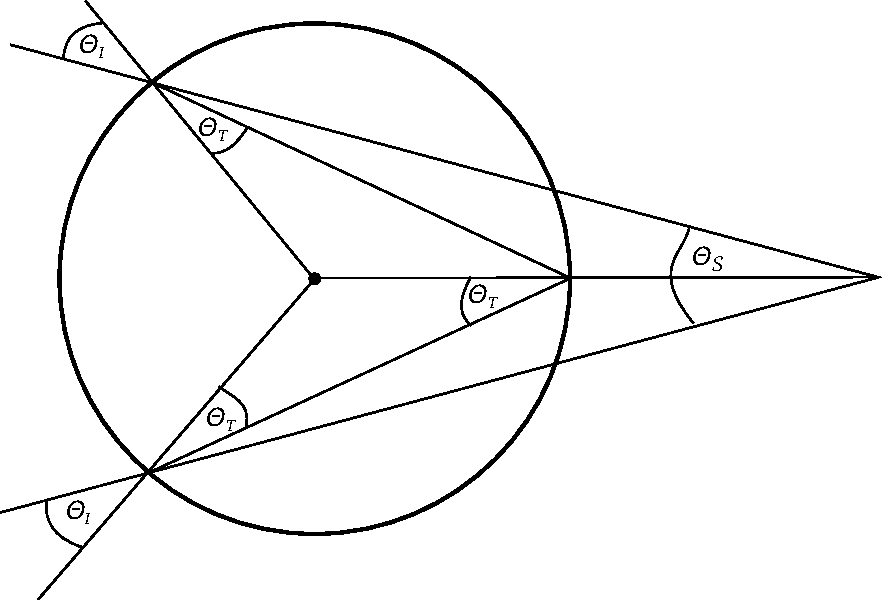
\includegraphics[width=\textwidth]{H2-Hauptregenbogen.pdf}
		\caption{Skizze zum Hauptregenbogen}
		\label{fig:haupt}
	\end{minipage}
	\begin{minipage}[b]{0.49\textwidth}
		\centering
		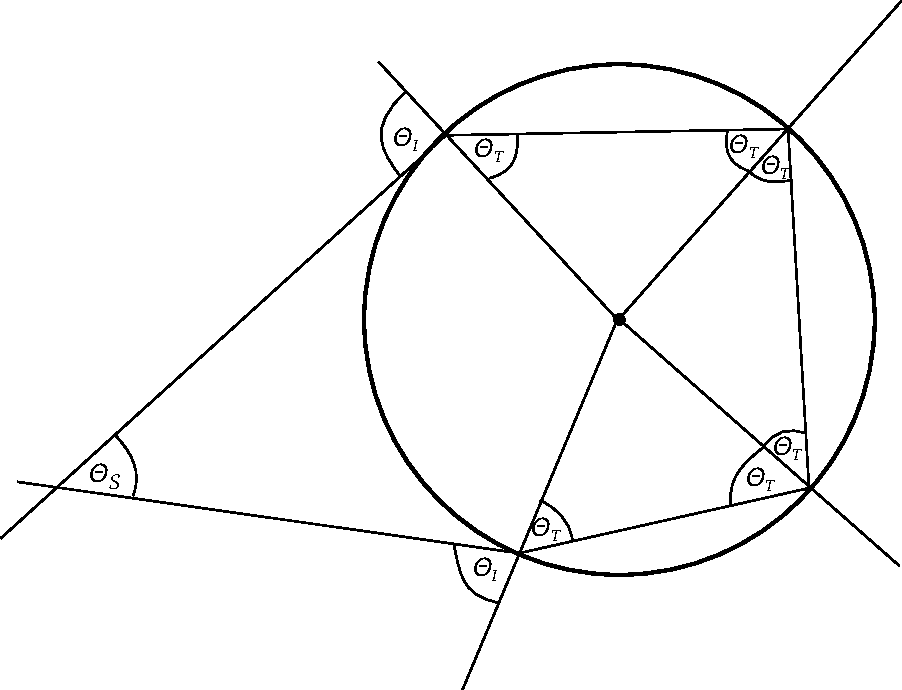
\includegraphics[width=\textwidth]{H2-Nebenregenbogen.pdf}
		\caption{Skizze zum Nebenregenbogen}
		\label{fig:neben}
	\end{minipage}
\end{figure}

Analog zur nächsten Aufgabe betrachten wir für den symmetrischen Fall, da wir
hier ein Extremum haben. Wir lesen aus der Skizze (Abbildung \ref{fig:haupt})
ab:
\[
	\half \Theta_S = \pi - \del{\Theta_I - \Theta_T} - \del{\pi - \Theta_T}
\]

Umgestellt:
\[
	\Theta_S = - 2 \Theta_I + 4 \Theta_T
\]

Wir setzen das Brechungsgesetz ein:
\[
	\Theta_S = - 2 \Theta_I + 4 \arcsin\del{\frac{\sin\del{\Theta_I}} n}
\]

Dann leiten wir ab:
\[
	\dod{\Theta_S}{\Theta_I} = \frac{4 \cos (\Theta_I)}{n \sqrt{1-\frac{\sin ^2(\Theta_I)}{n^2}}}-2 
\]

Dies setzen wir gleich 0 und formen nach $\Theta_I$ um. Wir erhalten:
\[
	\Theta_I = \arccos\del{\frac{\sqrt{n^2-1}}{\sqrt{3}}}
\]

Dann leiten wir noch einmal ab:
\[
	\dod[2]{\Theta_S}{\Theta_I} = 4 \left(\frac{\sin (\Theta_I) \cos ^2(\Theta_I)}{n^3 \left(1-\frac{\sin ^2(\Theta_I)}{n^2}\right)^{3/2}}-\frac{\sin (\Theta_I)}{n \sqrt{1-\frac{\sin ^2(\Theta_I)}{n^2}}}\right) 
\]

Wir setzen die Extremstelle $\Theta_I$ ein und erhalten:
\[
	-\frac{32 \sqrt{9-n^2}}{27 \sqrt{1-\frac{1}{n^2}} n}
\]

Zur Vorzeichenbestimmung setzen wir $n = 1.3$ ein und erhalten
$\unit{-3.85763}{\reciprocal\radian}$. Es handelt sich also um ein Maximum.

\subsection{Winkelbestimmung}

Wir gehen davon aus, dass sich bereits der extremale Winkel eingestellt hat.
Somit sind die Reflexionswinkel im Inneren alle gleich sowie -- wie auf der
Zeichnung auf dem Aufgabenblatt auch dargestellt -- der Austrittswinkel gleich
dem Eintrittswinkel. Das Fünfeck, das von den Lichtstrahlen aufgespannt wird
(siehe Abbildung \ref{fig:neben}), hat eine Winkelsumme von $3 \pi$. Es gilt
also:
\[
	\Theta_S = 3 \pi - 2 \del{\pi - \Theta_I} - 6 \Theta_T
	= \pi + 2 \Theta_I - 6 \Theta_T
\]

\subsection{Extremalbedingung}

Zuerst rechnen wir den Winkel um: $\Theta_S = \unit{0.891863}\radian$. Dann setzen wir das Brechungsgesetz in die Relation der vorherigen Aufgabe ein und erhalten:
\[
	\Theta_S = \pi + 2 \Theta_I - 6 \arcsin\del{\frac{\sin\del{\Theta_I}} n}
\]

Die leiten wir ab:
\[
	\dod{\Theta_S}{\Theta_I} = 2 - \frac{6 \cos{\del{\Theta_I}}}{n \sqrt{1 - \del{\frac{\sin\del{\Theta_I}}n}^2}}
\]

Und setzen gleich 0 und stellen nach $\Theta_I$ um:
\[
	\Theta_I = \pm \arccos\del{\pm \frac{\sqrt{-1 + n^2}}{2 \sqrt{2}}}
\]

Dabei interessiert uns nur die Lösung mit den zwei Pluszeichen. Wir setzen $n_B = 1.334$ und $n_R = 1.331$ ein und erhalten:
\[
	\Theta_I = \unit{0.937814}\radian
	,\quad
	\Theta_I = \unit{0.879037}\radian
\]

Mit einem Brechungsindex dazwischen würden wir auf die geforderten $\Theta_S = \unit{0.891863}\radian$ kommen.

Wir leiten noch einmal ab und erhalten:
\[
	\dod[2]{\Theta_S}{\Theta_I} = \frac{6 \left(n^2-1\right) \sin (\Theta_I)}{\sqrt{1-\frac{\sin ^2(\Theta_I)}{n^2}} \left(n^3-n \sin ^2(\Theta_I)\right)}
\]

Dort setzen wir die Extremstelle ein und erhalten:
\[
\frac{16 \sqrt{9-n^2}}{9 \sqrt{1-\frac{1}{n^2}} n}
\]

Für $n = 1.3$ erhalten wir $\unit{5.78644}{\reciprocal\radian}$, es handelt
sich also
um ein Minimum.

\subsection{Farbreihenfolge}

Da der Winkel ein Minimum und kein Maximum wie beim Primärbogen ist, ist die
\textcolor{red}F\textcolor{orange}a\textcolor{yellow}r\textcolor{green}b\textcolor{blue}reihenfolge
umgekehrt und somit ist \textcolor{blue}{rot} innen und \textcolor{red}{blau}
außen. Außerhalb des Bogens ist es auch heller als innerhalb. Das ganze sehen
wir auch an den Ergebnissen der vorherigen Aufgabe, denn
\textcolor{blue}{rotes} Licht wird weniger stark abgelenkt, der
\textcolor{blue}{rote} Bogen ist also kleiner, sprich innen.

%%%%%%%%%%%%%%%%%%%%%%%%%%%%%%%%%%%%%%%%%%%%%%%%%%%%%%%%%%%%%%%%%%%%%%%%%%%%%%%
%                  potentielle Energie eines Ionenkristalls                   %
%%%%%%%%%%%%%%%%%%%%%%%%%%%%%%%%%%%%%%%%%%%%%%%%%%%%%%%%%%%%%%%%%%%%%%%%%%%%%%%

\section{potentielle Energie eines Ionenkristalls}
\label 3

Das Durchzählen der Punkte ist relativ simpel realisiert, wir zählen alle
Punkte \[ \set{(x, y, z)\in \mathbb Z^3 \colon \max\set{x, y, z} \leq a} \]
durch. Dabei ist $a = 60$, wobei der Punkt $(0, 0, 0)$ ausgeschlossen worden
ist. Das Vorzeichen der Ladung an der Stelle $(x, y, z)$ haben wir durch
$(-1)^x (-1)^y (-1)^z = (-1)^{x+z+y}$ bestimmt. Somit ist der Ursprung, auf den
sich die potentielle Energie bezieht, in einer positiven Ladung zentriert.

Unser Programm für diese Aufgabe haben wir in Python 3 implementiert. Es kann
unter \\ \url{https://github.com/martin-ueding/physik321-08} (\texttt{H3.py})
heruntergeladen werden.

\inputminted[fontsize=\small, frame=lines, linenos]{python}{H3.py}

Die Ausgabe des Programms:

\inputminted[fontsize=\small, frame=lines]{text}{H3.py.txt}

Der Algorithmus hängt leider $\mathcal O\del{a^3}$ von der Eingabe ab, so dass
es ab $a = 60$ mehr als einige Sekunden dauert. Das Ergebnis ändert sich
allerdings nur noch wenig, für $a = 64$ haben wir $U =
\unit{-1.53015901663\e{-28}}\joule$ sowie für $a = 128$ haben wir $U =
\unit{-1.540450919\e{-28}}\joule$ erhalten. Für eine erste Abschätzung sollte
dies reichen.

Das ganze haben wir auch noch in C implementiert (\texttt{H3.c}, auch auf
GitHub):

\inputminted[fontsize=\small, frame=lines, linenos, tabsize=4]{c}{H3.c}

Die Ausgabe des Programms:

\inputminted[fontsize=\small, frame=lines]{text}{H3.c.txt}

Es kommt, von Rundungsfehlern abgesehen, das gleiche Ergebnis heraus. Auf
GitHub haben wir noch eine Version in Java, die mit $\unit{0.1}\second$ noch
einigermaßen zügig läuft.

%\bibliography{../../zentrale_BibTeX/Central}
%\bibliographystyle{plain}

\end{document}

% vim: spell spelllang=de
